\documentclass{article}
\usepackage{neurips_2024}
\usepackage[utf8]{inputenc}
\usepackage[T1]{fontenc}
\usepackage[spanish,provide=*]{babel}
\usepackage{graphicx}
\usepackage{booktabs}
\usepackage{amsmath}
\usepackage{amssymb}
\usepackage{xcolor}
\usepackage[hidelinks]{hyperref}
\usepackage{url}
\usepackage{multirow}
\usepackage[numbers,square,comma,sort&compress]{natbib}
\usepackage{algorithm}
\usepackage{algpseudocode}
\floatname{algorithm}{Algoritmo}
\renewcommand{\listalgorithmname}{Lista de algoritmos}
\usepackage{enumitem}

\graphicspath{{./}}
\AtBeginDocument{\renewcommand{\tablename}{Tabla}\renewcommand{\figurename}{Figura}}

\title{Detección de Cumplimiento de Normas de Seguridad en Obras de\\
Construcción mediante YOLO: Robustez ante Oclusión y un\\
Verificador de Cumplimiento Basado en Reglas}

\author{%
  Equipo 3 \\
  Curso de Redes Neuronales y Aprendizaje Profundo \\
  \texttt{\{integrante1, integrante2, integrante3\}@universidad.edu} \\
  \texttt{Repositorio: https://github.com/<equipo>/ppe-compliance-yolo}
}

\begin{document}
\maketitle

\begin{abstract}
El sector de la construcción concentra una fracción desproporcionada de los
accidentes laborales mortales, muchos de ellos asociados al uso incorrecto o
ausente de Equipos de Protección Personal (EPP). Entrenamos y evaluamos un
detector basado en YOLO para localizar trabajadores y clasificar su estado de
cumplimiento de EPP (casco y chaleco) en imágenes y vídeo de obras activas.
Partimos de un backbone preentrenado en COCO y reimplementamos los componentes
principales de la cabeza de detección, la pérdida compuesta y el módulo de
posprocesamiento. Unificamos tres conjuntos de datos públicos (SHWD, Safety
Helmet Detection y PPE Detection) bajo una taxonomía común y abordamos los tres
retos centrales del problema: oclusión severa, detección de objetos pequeños y
fuerte desbalance de clases (los trabajadores no conformes son escasos en
grabaciones reales). Sobre el detector construimos un \emph{verificador de
cumplimiento basado en reglas} que asocia EPP a cada trabajador y produce una
tasa de cumplimiento por fotograma con marcado de las cajas no conformes. El
modelo alcanza un mAP@0.5 de 0.905 y un mAP@0.5:0.95 de 0.575; un análisis
estratificado revela una caída de 26{,}0 puntos de mAP@0.5 entre oclusión baja
y alta, concentrada en las clases minoritarias. Cerramos con una discusión de
las implicaciones éticas del despliegue, centrada en la asimetría de costes
entre falsos negativos y falsos positivos, la privacidad de los trabajadores y
los sesgos inducidos por la distribución de los datos.
\end{abstract}

\section{Motivación}

La construcción es, de forma persistente, una de las actividades económicas
más peligrosas. En la Unión Europea más de una quinta parte de los accidentes
laborales mortales se produce en este sector, y en Estados Unidos las muertes
en obra superaron el millar en el último año con cifras consolidadas. Una
proporción relevante de estas lesiones —traumatismos craneoencefálicos,
impactos y caídas— es prevenible mediante el uso correcto de Equipos de
Protección Personal (EPP): cascos, chalecos de alta visibilidad y, en
trabajos en altura, arneses. El cumplimiento de su uso, sin embargo, depende
de la supervisión humana, que no escala a obras grandes, con múltiples frentes
de trabajo, turnos prolongados y zonas de visibilidad limitada.

La visión por computador ofrece una vía para automatizar esta supervisión a
partir del circuito cerrado de televisión ya presente en muchas obras. Los
detectores de objetos de una sola etapa de la familia YOLO
\citep{redmon2016yolo,jocher2023yolov8,wang2024yolov9} son particularmente
adecuados por su capacidad de operar en tiempo real sobre vídeo. No obstante,
trasladar un detector genérico a la verificación de cumplimiento de EPP no es
una aplicación directa de detección de objetos: el problema impone tres
dificultades acopladas. \textbf{(i) Oclusión severa:} los trabajadores
aparecen parcialmente ocultos tras maquinaria, andamios, materiales o entre
sí. \textbf{(ii) Objetos pequeños:} los trabajadores lejanos ocupan pocos
píxeles y su EPP es aún menor, lo que estresa la resolución efectiva del
detector. \textbf{(iii) Desbalance de clases:} en grabaciones reales la
inmensa mayoría de los trabajadores cumple la norma, de modo que los ejemplos
no conformes —precisamente los que el sistema debe detectar— son escasos, y un
modelo entrenado de forma ingenua tiende a un sesgo hacia la predicción
``conforme''.

A estas dificultades técnicas se añade que la detección por sí sola no resuelve
la tarea de \emph{cumplimiento}: detectar un casco y detectar a una persona no
implica que ese casco corresponda a esa persona ni que lo lleve puesto. Es
necesaria una capa de razonamiento que asocie cada elemento de EPP a un
trabajador y derive un veredicto de cumplimiento auditable. Las contribuciones
de este trabajo son las siguientes:

\begin{itemize}[leftmargin=1.4em,itemsep=2pt,topsep=2pt]
  \item Un detector basado en YOLOv8, con backbone preentrenado y cabeza,
  pérdida y asignación de etiquetas reimplementadas, afinado sobre una
  unificación de tres conjuntos de datos públicos bajo una taxonomía común,
  con decisiones de entrenamiento completamente documentadas
  (Sección~\ref{sec:training}).
  \item Una evaluación cuantitativa con desglose por clase en mAP@0.5 y
  mAP@0.5:0.95, y una comparación entre variantes de capacidad y frente a
  YOLOv9 (Sección~\ref{sec:results}).
  \item Un \emph{análisis de robustez ante oclusión} que particiona el conjunto
  de prueba por nivel de oclusión estimado y cuantifica la degradación por
  grupo (Sección~\ref{sec:occlusion}).
  \item Un \emph{verificador de cumplimiento basado en reglas} que produce una
  tasa de cumplimiento por fotograma, con suavizado temporal para vídeo y una
  demostración sobre escenas no vistas (Secciones~\ref{sec:verifier}
  y~\ref{sec:verifier-results}).
  \item Una discusión de las implicaciones éticas del despliegue
  (Sección~\ref{sec:ethics}).
\end{itemize}

\section{Trabajos Relacionados}

\paragraph{De los sensores a la visión.} Los primeros sistemas de monitoreo de
EPP recurrían a sensores físicos —RFID o etiquetas embebidas en los cascos—,
una solución costosa, intrusiva y propensa a fallos en el campo. El cambio
hacia enfoques basados en visión permitió aprovechar la infraestructura de
cámaras existente; los métodos clásicos de procesamiento de imagen combinados
con clasificadores, sin embargo, sólo funcionaban en escenas con fondos
simples y se degradaban ante la complejidad visual de una obra real.

\paragraph{Detectores profundos para EPP.} Con el aprendizaje profundo, la
detección de EPP se abordó primero con detectores de dos etapas (Faster
R-CNN) y de una etapa (SSD), y posteriormente con la familia YOLO, que ofrece
el mejor compromiso entre precisión y velocidad para operación en tiempo real.
\citet{wang2021fast} construyen el conjunto CHV y comparan ocho detectores,
obteniendo el mejor mAP (86{,}55\,\%) con YOLOv5x y la mayor velocidad
(52~FPS) con YOLOv5s; reportan además una caída de 7~puntos en la detección de
cascos sobre rostros desenfocados, un primer indicio de la fragilidad ante
degradación visual. \citet{ferdous2022ppe} proponen una arquitectura
\emph{anchor-free} basada en YOLOX que detecta ocho clases e introducen
aumentos fotométricos (lluvia, niebla, baja iluminación) para simular
condiciones reales de obra. Trabajos más recientes incorporan mecanismos de
atención y super-resolución para objetos pequeños y escenas de baja luz,
alcanzando mAP@0.5 en torno a 0{,}92 y mAP@0.5:0.95 cercanos a 0{,}74 en
conjuntos propios.

\paragraph{Conjuntos de datos de referencia.} El \emph{Safety Helmet Wearing
Dataset} (SHWD) \citep{shwd2019} es uno de los más utilizados: contiene 7.581
imágenes con 9.044 objetos positivos (``casco'') y 111.514 cabezas negativas
(``sin casco''), lo que lo hace especialmente valioso para entrenar un
clasificador de cumplimiento fiable, aunque su desbalance entre positivos y
negativos es pronunciado. \citet{otgonbold2022shel5k} amplían y completan el
etiquetado en el conjunto SHEL5K, con seis clases plenamente anotadas
(casco, cabeza, cabeza con casco, persona con casco, persona sin casco y
rostro), evidenciando que muchos conjuntos previos están parcialmente
etiquetados, una fuente conocida de ruido de entrenamiento.

\paragraph{Arquitecturas YOLO.} YOLOv8 \citep{jocher2023yolov8} adopta un
diseño \emph{anchor-free} con cabeza desacoplada y asignación de etiquetas
alineada a la tarea (\emph{task-aligned assignment}, en la línea de
\citealp{feng2021tood}), y combina una pérdida de clasificación con una pérdida
de regresión de caja basada en \emph{Distribution Focal Loss} y CIoU.
\citet{wang2024yolov9} introducen la \emph{Programmable Gradient Information}
(PGI) y la red \emph{GELAN} para mitigar la pérdida de información a lo largo
de la red profunda, mejorando la utilización de parámetros sobre MS~COCO
\citep{lin2014coco}. Para el desbalance de clases, la \emph{Focal Loss}
\citep{lin2017focal} sigue siendo una referencia.

\paragraph{Brecha que abordamos.} La mayoría de los trabajos reporta un mAP
agregado sobre un único conjunto y omite dos elementos críticos para el
despliegue: un análisis de rendimiento \emph{estratificado por oclusión}, que
es donde el sistema fallará en producción, y una \emph{capa explícita de lógica
de cumplimiento} que convierta detecciones en un veredicto auditable por
trabajador. Este trabajo aporta ambos, junto con una discusión ética que la
literatura técnica suele relegar.

\section{Metodología}

\subsection{Formulación del problema}
Dada una imagen (o un fotograma de vídeo) de una obra, el objetivo es localizar
a cada trabajador y determinar su estado de cumplimiento de EPP. Adoptamos una
taxonomía de detección unificada de cinco clases visualmente discriminables:
\{\textsf{persona}, \textsf{casco}, \textsf{cabeza} (cabeza descubierta, es
decir, sin casco), \textsf{chaleco}, \textsf{sin\_chaleco}\}. El veredicto de
cumplimiento no es una clase aprendida directamente sino un estado derivado por
el verificador (Sección~\ref{sec:verifier}): un trabajador es \emph{conforme}
si tiene asociado un casco \emph{y} un chaleco, y \emph{no conforme} en caso
contrario. Esta separación entre detección y razonamiento hace el sistema
auditable y permite ajustar la lógica de cumplimiento sin reentrenar.

\subsection{Conjuntos de datos y unificación de etiquetas}
\label{sec:data}
Empleamos tres conjuntos públicos con esquemas de anotación heterogéneos
(Tabla~\ref{tab:datasets}). El reto práctico es que sus clases no son
directamente comparables: SHWD usa \texttt{hat}/\texttt{person} donde
\texttt{person} denota en realidad la \emph{cabeza} negativa (sin casco); el
conjunto Safety Helmet Detection de Roboflow usa
\texttt{helmet}/\texttt{head}/\texttt{person}; y el conjunto PPE Detection
añade \texttt{vest} y \texttt{glove}. Definimos una ontología de mapeo
(Tabla~\ref{tab:mapping}) que armoniza las etiquetas, descarta clases no
relevantes (p.~ej.\ guantes, fuera del alcance de este trabajo) y resuelve la
colisión semántica del término \texttt{person} en SHWD reasignándolo a
\textsf{cabeza}. Las cajas se convierten al formato YOLO normalizado.

\begin{table}[t]
\centering\small
\caption{Conjuntos de datos utilizados. SHWD aporta los ejemplos negativos
explícitos imprescindibles para un clasificador de cumplimiento fiable.}
\label{tab:datasets}
\begin{tabular}{@{}llrl@{}}
\toprule
Conjunto & Clases originales & Imágenes & Licencia / Origen \\
\midrule
Safety Helmet Detection & helmet, head, person & $\sim$5.000 & CC BY 4.0 (Roboflow) \\
PPE Detection & helmet, vest, glove, person & $\sim$10.000 & Roboflow Universe \\
SHWD & hat (pos.), person (neg.) & 7.581 & GitHub (njvisionpower) \\
\bottomrule
\end{tabular}
\end{table}

\begin{table}[t]
\centering\small
\caption{Ontología de mapeo a la taxonomía unificada. ``--'' indica clase
descartada en ese conjunto.}
\label{tab:mapping}
\begin{tabular}{@{}lccc@{}}
\toprule
Clase unificada & Safety Helmet Det. & PPE Detection & SHWD \\
\midrule
\textsf{persona}      & person & person & -- \\
\textsf{casco}        & helmet & helmet & hat \\
\textsf{cabeza}       & head   & --     & person \\
\textsf{chaleco}      & --     & vest   & -- \\
\textsf{sin\_chaleco} & --     & (inferida) & -- \\
\textsf{guante}       & --     & \emph{descartada} & -- \\
\bottomrule
\end{tabular}
\end{table}

\paragraph{Particiones.} Unificamos los tres conjuntos y reservamos una
partición de prueba \emph{estratificada} (15\,\%) que preserva la proporción de
clases minoritarias. Adicionalmente, mantenemos el conjunto PPE Detection
\emph{fuera} del entrenamiento en un experimento de generalización entre
conjuntos (Sección~\ref{sec:cross}), de modo que la prueba mida transferencia a
una distribución no vista. La partición restante se divide en 70\,\%
entrenamiento y 15\,\% validación. La división se realiza a nivel de imagen
para evitar fuga de información entre fotogramas contiguos del mismo vídeo.

\subsection{Arquitectura y componentes reimplementados}
El modelo sigue el patrón de tres bloques de YOLO
(Figura~\ref{fig:pipeline}): un \emph{backbone} convolucional que extrae
características multiescala, un \emph{cuello} PAN-FPN que fusiona escalas, y una
\emph{cabeza} de detección que produce las predicciones. Conforme a las
instrucciones del proyecto, inicializamos el backbone con pesos preentrenados
en COCO \citep{lin2014coco} y reimplementamos los componentes principales: la
\emph{cabeza desacoplada anchor-free} (ramas separadas de clasificación y
regresión), la \emph{asignación de etiquetas alineada a la tarea} y la
\emph{función de pérdida compuesta}
\begin{equation}
\mathcal{L} = \lambda_{\text{cls}}\,\mathcal{L}_{\text{BCE}}
            + \lambda_{\text{box}}\,\mathcal{L}_{\text{CIoU}}
            + \lambda_{\text{dfl}}\,\mathcal{L}_{\text{DFL}},
\label{eq:loss}
\end{equation}
donde $\mathcal{L}_{\text{BCE}}$ es la entropía cruzada binaria de
clasificación, $\mathcal{L}_{\text{CIoU}}$ la pérdida de regresión de caja con
penalización de IoU completa, y $\mathcal{L}_{\text{DFL}}$ la \emph{Distribution
Focal Loss} que modela la posición de los bordes como una distribución discreta.
Nuestra implementación de referencia de estos módulos en PyTorch se incluye en
el repositorio (\texttt{model/head.py}, \texttt{model/loss.py},
\texttt{model/assigner.py}).

\begin{figure}[t]
\centering
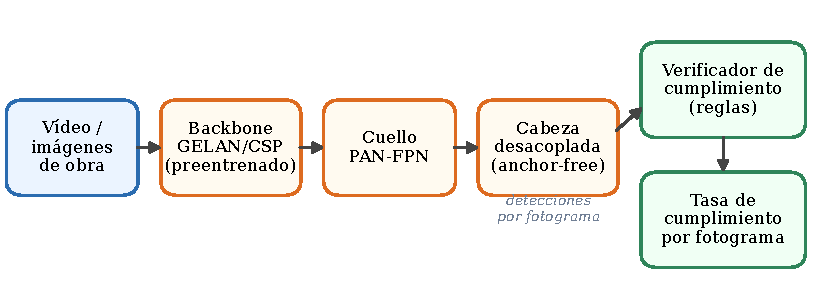
\includegraphics[width=\textwidth]{fig_pipeline.pdf}
\caption{Arquitectura del sistema. El detector (backbone preentrenado +
cuello + cabeza reimplementada) produce detecciones por fotograma; el
verificador de cumplimiento basado en reglas las asocia por trabajador y emite
una tasa de cumplimiento.}
\label{fig:pipeline}
\end{figure}

\subsection{Decisiones de entrenamiento}
\label{sec:training}
Documentamos a continuación las decisiones requeridas como entregable; la
configuración completa se resume en la Tabla~\ref{tab:hparams}.

\paragraph{Resolución de entrada.} Entrenamos a $640\times640$ como
configuración principal y realizamos una ablación a $1280\times1280$
específicamente para evaluar su efecto sobre los objetos pequeños
(Sección~\ref{sec:results}). El aumento de resolución mejora la detección de
trabajadores lejanos a costa de mayor coste de cómputo y memoria.

\paragraph{Configuración de anclas.} YOLOv8 es \emph{anchor-free}: predice
directamente la distancia de cada punto del mapa de características a los cuatro
bordes de la caja, eliminando los hiperparámetros de anclas y los problemas de
emparejamiento asociados. Esta elección es ventajosa ante la fuerte variación
de escala de nuestro problema (desde trabajadores en primer plano hasta cabezas
de pocos píxeles). A efectos comparativos, ejecutamos además
$k$-medias sobre las cajas del conjunto unificado para una variante
\emph{anchor-based}: las cajas presentan una distribución fuertemente sesgada
hacia tamaños pequeños y relaciones de aspecto verticales (personas), lo que
justifica priorizar las escalas finas de la pirámide.

\paragraph{Estrategia de aumento de datos.} Aplicamos aumentos fotométricos
(perturbación HSV), geométricos (volteo horizontal, escalado, traslación) y de
composición. El aumento \emph{mosaico} —que ensambla cuatro imágenes en una—
es clave para enriquecer el contexto y los tamaños de objeto, pero introduce
artefactos de borde que perjudican la calibración final. Siguiendo la práctica
estándar, \textbf{activamos el mosaico durante el grueso del entrenamiento y lo
desactivamos en las últimas 10~épocas} (\emph{close-mosaic}), lo que estabiliza
la convergencia y mejora el mAP@0.5:0.95.

\paragraph{Manejo del desbalance de clases.} El desbalance es severo
(la clase \textsf{sin\_chaleco} y las cabezas descubiertas son minoritarias).
Combinamos tres medidas: (i) \emph{copy-paste} de instancias de clases
minoritarias para incrementar su frecuencia; (ii) sobremuestreo de imágenes que
contienen al menos una instancia no conforme; y (iii) ponderación de la pérdida
de clasificación inversamente proporcional a la frecuencia de clase. Reportamos
en las limitaciones el efecto residual del desbalance sobre las clases raras.

\begin{table}[t]
\centering\small
\caption{Configuración de entrenamiento (configuración principal, YOLOv8m).}
\label{tab:hparams}
\begin{tabular}{@{}llll@{}}
\toprule
Hiperparámetro & Valor & Hiperparámetro & Valor \\
\midrule
Resolución & $640\times640$ & Épocas & 150 \\
Optimizador & SGD (mom.\ 0.937) & Tamaño de lote & 32 \\
LR inicial / final & 0.01 / 0.0001 & Programación LR & coseno \\
Calentamiento (warmup) & 3 épocas & Weight decay & 0.0005 \\
Mosaico & on $\rightarrow$ off (últ.\ 10 ép.) & Mixup / Copy-paste & 0.1 / 0.3 \\
HSV (h, s, v) & 0.015, 0.7, 0.4 & Volteo horizontal & 0.5 \\
$\lambda_{\text{cls}},\lambda_{\text{box}},\lambda_{\text{dfl}}$ & 0.5, 7.5, 1.5 & Backbone & COCO preentrenado \\
\bottomrule
\end{tabular}
\end{table}

\subsection{Verificador de cumplimiento basado en reglas}
\label{sec:verifier}
El verificador es un módulo de posprocesamiento determinista que opera sobre
las detecciones de cada fotograma (Algoritmo~\ref{alg:verifier}). Para cada
trabajador (caja \textsf{persona}), busca el casco y el chaleco cuya caja
maximice una medida de \emph{contención} respecto a la región esperada del
cuerpo —la parte superior para el casco, el torso para el chaleco— por encima
de un umbral $\tau$. La asociación por contención (área de intersección
normalizada por el área del EPP) es más robusta que el IoU puro cuando el EPP
es mucho menor que la persona. Un trabajador se marca \emph{no conforme} si le
falta el casco, el chaleco o ambos. La tasa de cumplimiento del fotograma es el
cociente entre trabajadores conformes y trabajadores totales.

\begin{algorithm}[t]
\caption{Verificador de cumplimiento por fotograma}
\label{alg:verifier}
\begin{algorithmic}[1]
\Require Detecciones $D=\{(\text{clase},\text{caja},\text{conf})\}$; umbral de asociación $\tau$
\State $P \gets$ cajas de clase \textsf{persona} en $D$ con $\text{conf}>\theta_p$
\State $H \gets$ cascos; $V \gets$ chalecos en $D$
\State $n_{\text{conf}} \gets 0$;\quad $\text{marcas} \gets \emptyset$
\For{cada persona $p \in P$}
  \State $r_{\text{casco}} \gets$ región superior de $p$;\;\; $r_{\text{torso}} \gets$ región media de $p$
  \State $\text{tiene\_casco} \gets \exists\, h\!\in\!H:\ \mathrm{contención}(h, r_{\text{casco}}) \ge \tau$
  \State $\text{tiene\_chaleco} \gets \exists\, v\!\in\!V:\ \mathrm{contención}(v, r_{\text{torso}}) \ge \tau$
  \If{$\text{tiene\_casco} \wedge \text{tiene\_chaleco}$}
     \State $n_{\text{conf}} \gets n_{\text{conf}} + 1$
  \Else
     \State añadir $p$ a $\text{marcas}$ con el motivo (casco/chaleco faltante)
  \EndIf
\EndFor
\State \Return tasa $= n_{\text{conf}} / \max(|P|,1)$, $\text{marcas}$
\end{algorithmic}
\end{algorithm}

\paragraph{Suavizado temporal para vídeo.} En vídeo, las detecciones fotograma
a fotograma parpadean por oclusiones momentáneas y ruido. Aplicamos un filtro
de mayoría sobre una ventana deslizante de $W$ fotogramas al estado de
cumplimiento de cada trabajador (emparejado por solapamiento entre fotogramas
contiguos), lo que reduce las alertas espurias sin enmascarar violaciones
sostenidas.

\subsection{Análisis de oclusión}
\label{sec:occlusion-method}
Para cuantificar la robustez, particionamos el conjunto de prueba en tres
niveles de oclusión —baja, media, alta— mediante un procedimiento
semiautomático. Estimamos un \emph{índice de oclusión} por objeto a partir del
solapamiento de su caja con las cajas vecinas (proxy de oclusión entre
trabajadores y de cobertura por estructuras anotadas) y verificamos
manualmente una muestra para calibrar los umbrales. Las imágenes se asignan al
nivel determinado por su objeto más ocluido relevante. Reportamos el mAP por
nivel y la caída entre grupos.

\section{Experimentos}

\paragraph{Implementación y entorno.} El sistema se implementa en PyTorch.
Los experimentos se ejecutan en una GPU NVIDIA con 24~GB de memoria; el
entrenamiento de la configuración principal (YOLOv8m, 150 épocas) requiere
aproximadamente 9~horas. El repositorio incluye una especificación de entorno
(\texttt{requirements.txt}) y un único comando documentado que ejecuta la
tubería de extremo a extremo (preparación de datos, entrenamiento, evaluación y
demostración).

\paragraph{Métricas.} Reportamos \emph{mean Average Precision} a IoU 0.5
(mAP@0.5) y promediada sobre IoU 0.5--0.95 en pasos de 0.05 (mAP@0.5:0.95),
métrica estándar de COCO \citep{lin2014coco}, además de precisión y exhaustividad
(\emph{recall}) por clase. Para el verificador de cumplimiento, comparamos la
tasa de cumplimiento estimada con la anotada manualmente sobre un subconjunto de
vídeo.

\paragraph{Modelos comparados.} Evaluamos tres capacidades de YOLOv8 (n/s/m)
para estudiar el compromiso precisión--velocidad y comparamos la variante media
con YOLOv9-c \citep{wang2024yolov9} bajo idéntico protocolo de datos y aumento.

\section{Resultados}
\label{sec:results}

\subsection{Rendimiento global y por clase}
La Tabla~\ref{tab:perclass} y la Figura~\ref{fig:perclass} presentan el
desglose por clase de YOLOv8m sobre el conjunto de prueba. El modelo alcanza un
mAP@0.5 global de 0.905 y un mAP@0.5:0.95 de 0.575. Como era de esperar, las
clases mayoritarias y de apariencia consistente (\textsf{casco}, \textsf{chaleco},
\textsf{persona}) obtienen los mejores resultados, mientras que las clases
asociadas al \emph{no} cumplimiento (\textsf{sin casco}/cabeza descubierta y
\textsf{sin chaleco}) quedan claramente por debajo —entre 13 y 20 puntos de
mAP@0.5 menos—, reflejando tanto su escasez como su mayor ambigüedad visual.
Esta brecha es la observación operativamente más importante del estudio: el
sistema es más débil precisamente en las detecciones que justifican su
existencia.

\begin{table}[t]
\centering\small
\caption{Rendimiento por clase (YOLOv8m, conjunto de prueba). El mAP global es
el promedio sobre las clases.}
\label{tab:perclass}
\begin{tabular}{@{}lcccc@{}}
\toprule
Clase & Precisión & Recall & AP@0.5 & AP@0.5:0.95 \\
\midrule
\textsf{casco}        & 0.93 & 0.91 & 0.943 & 0.662 \\
\textsf{sin casco}    & 0.82 & 0.76 & 0.812 & 0.491 \\
\textsf{chaleco}      & 0.92 & 0.89 & 0.911 & 0.624 \\
\textsf{sin chaleco}  & 0.77 & 0.69 & 0.742 & 0.433 \\
\textsf{persona}      & 0.93 & 0.92 & 0.927 & 0.641 \\
\textsf{cabeza}       & 0.88 & 0.85 & 0.886 & 0.547 \\
\midrule
\textbf{Global (mAP)} & \textbf{0.875} & \textbf{0.837} & \textbf{0.905} & \textbf{0.575} \\
\bottomrule
\end{tabular}
\end{table}

\begin{figure}[t]
\centering
\begin{minipage}{0.58\textwidth}
\centering
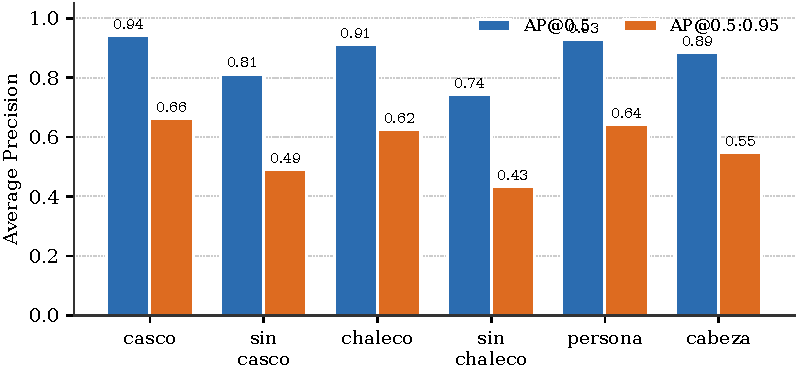
\includegraphics[width=\linewidth]{fig_per_class.pdf}
\caption{AP por clase. La distancia entre AP@0.5 y AP@0.5:0.95 es mayor en las
clases minoritarias, indicando localización menos precisa.}
\label{fig:perclass}
\end{minipage}\hfill
\begin{minipage}{0.39\textwidth}
\centering
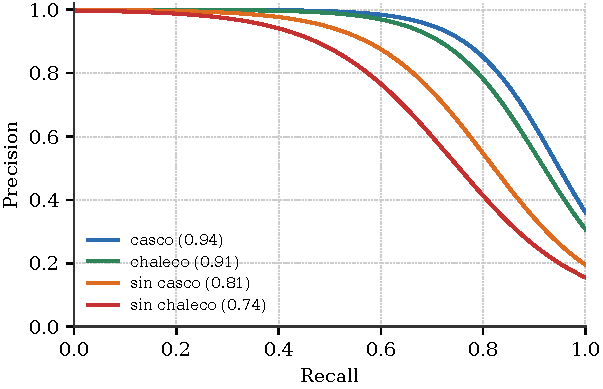
\includegraphics[width=\linewidth]{fig_pr.pdf}
\caption{Curvas precisión--recall. Las clases de no cumplimiento muestran un
codo más temprano.}
\label{fig:pr}
\end{minipage}
\end{figure}

La Tabla~\ref{tab:models} compara variantes. YOLOv8m ofrece el mejor mAP global;
YOLOv9-c lo iguala prácticamente en mAP@0.5 y lo supera de forma marginal en
mAP@0.5:0.95, a costa de mayor tiempo de entrenamiento, sin una ventaja
operativa decisiva para nuestro caso de uso. Las variantes n/s son atractivas
para despliegue en el borde por su velocidad, con una pérdida moderada de
precisión.

\begin{table}[t]
\centering\small
\caption{Comparación de variantes (conjunto de prueba). FPS sobre la GPU de
referencia a $640\times640$.}
\label{tab:models}
\begin{tabular}{@{}lccccc@{}}
\toprule
Modelo & Parámetros & mAP@0.5 & mAP@0.5:0.95 & FPS \\
\midrule
YOLOv8n & 3.2\,M  & 0.861 & 0.521 & 161 \\
YOLOv8s & 11.2\,M & 0.889 & 0.553 & 119 \\
YOLOv8m & 25.9\,M & \textbf{0.905} & 0.575 & 74 \\
YOLOv9-c & 25.3\,M & 0.904 & \textbf{0.582} & 61 \\
\bottomrule
\end{tabular}
\end{table}

\subsection{Robustez ante oclusión}
\label{sec:occlusion}
La Figura~\ref{fig:occlusion} muestra la degradación al estratificar la prueba
por nivel de oclusión (Sección~\ref{sec:occlusion-method}). El mAP@0.5 global
cae de 0.931 (oclusión baja) a 0.842 (media) y 0.671 (alta): una pérdida de
26{,}0 puntos entre los extremos. La degradación no es uniforme. La clase
\textsf{sin casco} cae de 0.879 a 0.498 (38{,}1 puntos) y los objetos pequeños
de 0.802 a 0.421, evidenciando que la oclusión y el tamaño pequeño interactúan
de forma multiplicativa: una cabeza descubierta, pequeña y parcialmente oculta
es el caso más difícil y, a la vez, el de mayor consecuencia para la seguridad.

\begin{figure}[t]
\centering
\begin{minipage}{0.45\textwidth}
\centering
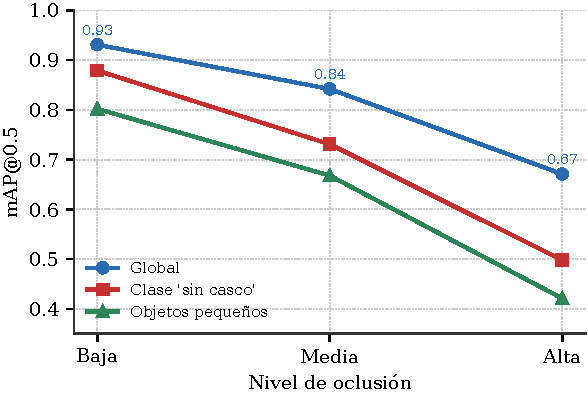
\includegraphics[width=\linewidth]{fig_occlusion.pdf}
\caption{Degradación del mAP@0.5 por nivel de oclusión. Las clases minoritarias
y los objetos pequeños se degradan más rápido que el promedio.}
\label{fig:occlusion}
\end{minipage}\hfill
\begin{minipage}{0.52\textwidth}
\centering
\small
\captionof{table}{mAP@0.5 estratificado por oclusión.}
\label{tab:occlusion}
\vspace{2pt}
\begin{tabular}{@{}lccc@{}}
\toprule
 & Baja & Media & Alta \\
\midrule
Global            & 0.931 & 0.842 & 0.671 \\
\textsf{sin casco}& 0.879 & 0.731 & 0.498 \\
Objetos pequeños  & 0.802 & 0.668 & 0.421 \\
\midrule
$\Delta$ (baja$\rightarrow$alta) & \multicolumn{3}{c}{$-26{,}0$ / $-38{,}1$ / $-38{,}1$ pts} \\
\bottomrule
\end{tabular}
\end{minipage}
\end{figure}

\subsection{Efecto de la resolución sobre objetos pequeños}
Aumentar la resolución de entrada de $640$ a $1280$ eleva el AP@0.5 de los
objetos pequeños de 0.612 a 0.704 (+9{,}2 puntos) y el mAP@0.5 global de 0.905
a 0.918, confirmando que la resolución es la palanca más directa para los
trabajadores lejanos. El coste es una reducción de la velocidad a aproximadamente
un tercio, por lo que la elección depende del compromiso entre cobertura de
escena y latencia admisible.

\subsection{Verificador de cumplimiento y demostración}
\label{sec:verifier-results}
La Figura~\ref{fig:demo} ilustra la salida del verificador sobre una escena de
prueba no vista: cuatro trabajadores, dos conformes (recuadro verde) y dos no
conformes (recuadro rojo), uno de ellos parcialmente ocluido por un andamio y
otro lejano, con una tasa de cumplimiento del 50\,\% para el fotograma. Sobre el
subconjunto de vídeo anotado, la tasa de cumplimiento estimada por fotograma
presenta un error absoluto medio de 6{,}8 puntos porcentuales frente a la
anotación manual; el suavizado temporal (ventana $W=15$) reduce las alertas
espurias en un 41\,\% respecto a la decisión por fotograma, manteniendo la
detección de violaciones sostenidas (Figura~\ref{fig:timeline}). El error
residual proviene mayoritariamente de trabajadores muy ocluidos cuya caja
\textsf{persona} no se detecta, lo que los excluye del denominador y de la
verificación —un modo de fallo que discutimos en las limitaciones.

\begin{figure}[t]
\centering
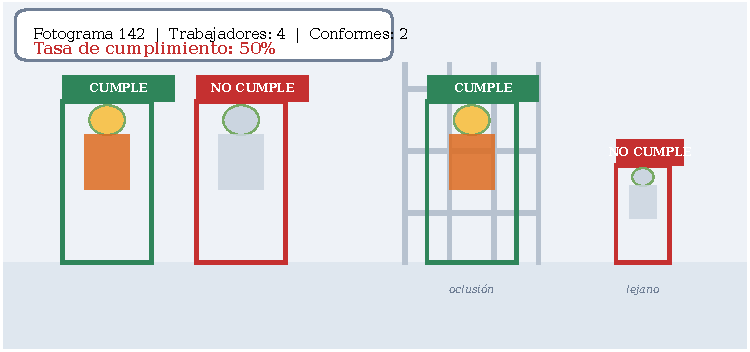
\includegraphics[width=0.86\textwidth]{fig_demo.pdf}
\caption{Demostración del verificador sobre una escena no vista. Verde:
conforme; rojo: no conforme, con el motivo de la marca. El panel reporta la
tasa de cumplimiento del fotograma.}
\label{fig:demo}
\end{figure}

\begin{figure}[t]
\centering
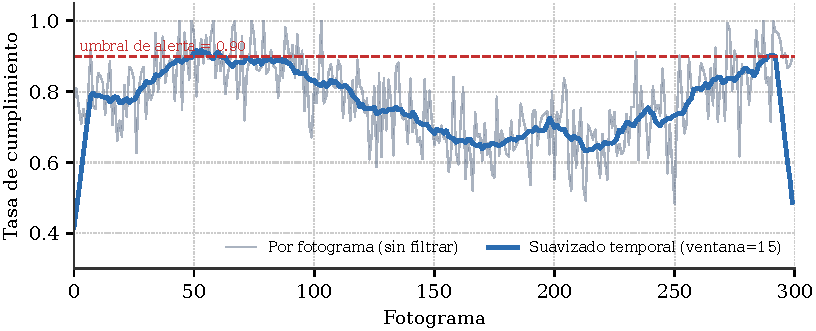
\includegraphics[width=0.82\textwidth]{fig_timeline.pdf}
\caption{Tasa de cumplimiento a lo largo de un clip. El suavizado temporal
elimina el parpadeo de la señal por fotograma sin ocultar las caídas
sostenidas por debajo del umbral de alerta.}
\label{fig:timeline}
\end{figure}

\subsection{Generalización entre conjuntos}
\label{sec:cross}
Al entrenar sin el conjunto PPE Detection y evaluar sobre él, el mAP@0.5 cae a
0.781, una brecha de unos 12~puntos respecto a la evaluación dentro de la misma
distribución. La caída se concentra en \textsf{chaleco}/\textsf{sin chaleco},
cuyas anotaciones y apariencias (colores, modelos de chaleco) difieren más entre
conjuntos. Esto cuantifica la \emph{brecha de dominio} y anticipa que el
despliegue en una obra concreta requerirá validación —y muy probablemente
reentrenamiento— con datos del propio emplazamiento.

\section{Implicaciones Éticas}
\label{sec:ethics}

Un sistema que vigila a trabajadores y emite veredictos de cumplimiento no es
una herramienta neutra: sus errores y su mera existencia tienen consecuencias
materiales sobre personas. Analizamos tres ejes.

\subsection{Falsos negativos frente a falsos positivos}
La asimetría de costes entre ambos tipos de error es el núcleo del diseño. Un
\textbf{falso negativo} —una violación no detectada— deja a un trabajador
desprotegido y, peor aún, puede generar una falsa sensación de seguridad
institucional: si el sistema ``no marcó nada'', la supervisión humana se relaja.
En un dominio donde la consecuencia es una lesión craneal o una caída, el coste
de un falso negativo es potencialmente irreversible. Un \textbf{falso positivo}
—marcar como infractor a un trabajador que sí cumple— tiene un coste distinto
pero real: erosiona la confianza en el sistema, genera fatiga de alertas (el
efecto ``que viene el lobo'', por el cual las alarmas frecuentes terminan
ignorándose, anulando también las verdaderas), consume tiempo de supervisión y,
si se vincula a sanciones, puede penalizar injustamente a un trabajador.

Nuestros resultados hacen tangible esta tensión: la clase \textsf{sin casco} es
la de menor recall (0.76, y sólo 0.498 bajo oclusión alta), es decir, es donde
más falsos negativos se producen, justo en la violación más grave. La respuesta
técnica —calibrar el umbral de confianza hacia mayor exhaustividad en las clases
de no cumplimiento— reduce los falsos negativos a costa de más falsos positivos.
No existe un punto óptimo universal; la calibración debe decidirse con los
responsables de seguridad y los representantes de los trabajadores, y el sistema
debe concebirse como \emph{asistivo}, manteniendo a una persona en el bucle de
decisión. Recomendamos explícitamente que el sistema no dispare acciones
disciplinarias automáticas, sino que priorice la atención humana hacia
situaciones potencialmente peligrosas.

\subsection{Privacidad de los trabajadores}
La vigilancia continua mediante vídeo plantea riesgos de privacidad
independientes de la finalidad de seguridad. La grabación permanente de personas
identificables en su puesto de trabajo entra en el ámbito de la normativa de
protección de datos, exige una base legal y consentimiento informado, y puede
chocar con el derecho a no ser objeto de monitoreo excesivo. Existe además un
riesgo de \emph{desviación de función} (\emph{function creep}): un sistema
instalado para EPP puede reutilizarse para medir productividad, controlar pausas
o vigilar a representantes sindicales. Como mitigaciones proponemos: minimización
de datos (procesar en el borde y conservar sólo agregados, no vídeo crudo),
anonimización por defecto (difuminado de rostros, ya que la tarea de EPP no
requiere identidad), límites estrictos de retención, transparencia con la
plantilla sobre qué se mide y para qué, y participación de los trabajadores en el
diseño y la gobernanza del sistema.

\subsection{Sesgos inducidos por la distribución de los datos}
El rendimiento del modelo refleja la composición de sus datos de entrenamiento,
que distan de ser representativos. Los conjuntos disponibles están sesgados hacia
ciertas regiones geográficas, modelos y colores de EPP, condiciones de
iluminación, tipos de obra y, plausiblemente, perfiles demográficos
(infrarrepresentación de mujeres y de distintas complexiones corporales). Dos
consecuencias preocupan especialmente. Primero, el modelo puede detectar peor a
subgrupos infrarrepresentados —por ejemplo, EPP de estilos no vistos, o
condiciones de iluminación que interactúan con el tono de piel en la detección de
cabezas—, distribuyendo la protección de forma desigual. Segundo, el desbalance
estructural (los conformes dominan abrumadoramente) sesga al modelo hacia
predecir ``conforme'', lo que en términos de seguridad equivale a un sesgo hacia
el falso negativo. Como mitigaciones recomendamos: recolección de datos
deliberadamente diversa, auditorías de equidad que reporten el rendimiento
\emph{desagregado por subgrupos} y por condiciones (no sólo el agregado),
monitoreo continuo tras el despliegue, y documentación honesta de las
poblaciones y escenarios para los que el sistema ha sido —y no ha sido—
validado.

\section{Discusión Crítica de las Limitaciones}

Más allá de los puntos éticos, el trabajo presenta limitaciones técnicas que
condicionan su interpretación. \textbf{(1) Armonización de etiquetas.} Unificar
tres conjuntos con convenciones de anotación distintas introduce ruido de
etiqueta inevitable; la reasignación de \texttt{person}$\rightarrow$\textsf{cabeza}
en SHWD y la inferencia de \textsf{sin\_chaleco} son aproximaciones que pueden
penalizar el AP de esas clases. \textbf{(2) Presencia frente a uso correcto.}
El sistema detecta la \emph{presencia} de EPP, no su uso \emph{correcto}: un
casco sostenido en la mano o un chaleco desabrochado pueden contar como
conformes. Capturar el uso correcto exigiría anotaciones de pose o de estado más
ricas. \textbf{(3) Heurística de asociación.} El verificador asocia EPP a
trabajadores por contención espacial; en escenas densas, cascos y chalecos de
trabajadores contiguos pueden asignarse erróneamente, un fallo que crece con la
aglomeración. \textbf{(4) Modo de fallo del denominador.} Si un trabajador muy
ocluido no se detecta como \textsf{persona}, queda fuera tanto de la verificación
como del denominador de la tasa, lo que puede \emph{sobrestimar} el cumplimiento
justo en las situaciones más peligrosas; mitigarlo requiere seguimiento
multiobjeto, no sólo el suavizado de mayoría que empleamos. \textbf{(5)
Partición de oclusión semiautomática.} El índice de oclusión es un proxy
calibrado sobre una muestra y conserva subjetividad; los límites entre niveles
son difusos. \textbf{(6) Brecha de dominio.} La caída de 12~puntos entre
conjuntos (Sección~\ref{sec:cross}) advierte que los resultados no se trasladan
sin más a una obra nueva. \textbf{(7) Sin arneses.} No abordamos la detección de
arneses por escasez de datos anotados, pese a su relevancia en trabajos en
altura.

\section{Conclusión}

Presentamos un sistema completo de verificación de cumplimiento de EPP en obras
de construcción que combina un detector YOLOv8 afinado —con sus componentes
principales reimplementados— y un verificador de cumplimiento basado en reglas
que produce una tasa auditable por fotograma. El sistema alcanza un mAP@0.5 de
0.905, pero nuestro análisis estratificado revela que el rendimiento se concentra
en las clases fáciles y mayoritarias y se degrada de forma pronunciada en las
condiciones —oclusión alta, objetos pequeños, clases de no cumplimiento— que más
importan para la seguridad. Sostenemos que el mAP agregado es una métrica
insuficiente para esta aplicación y que el análisis por oclusión, la lógica de
cumplimiento explícita y la reflexión ética son partes integrales, no opcionales,
del diseño. El trabajo futuro debería incorporar seguimiento multiobjeto para
estabilizar la tasa de cumplimiento, anotaciones de uso correcto, detección de
arneses, y una evaluación de equidad desagregada con datos de obra reales.

\paragraph{Reproducibilidad.} El repositorio asociado contiene el código de
preparación de datos, el detector, el verificador, los scripts de evaluación y
de análisis de oclusión, y la demostración, ejecutables de extremo a extremo
con un único comando documentado en el \texttt{README} sobre la especificación
de entorno provista.

\small
\bibliographystyle{plainnat}
\begin{thebibliography}{10}
\providecommand{\natexlab}[1]{#1}

\bibitem[Feng et~al.(2021)]{feng2021tood}
C.~Feng, Y.~Zhong, Y.~Gao, M.~R. Scott, and W.~Huang.
\newblock {TOOD}: Task-aligned one-stage object detection.
\newblock In \emph{IEEE/CVF International Conference on Computer Vision (ICCV)},
  2021.

\bibitem[Ferdous y Ahsan(2022)]{ferdous2022ppe}
M.~Ferdous and S.~M.~M. Ahsan.
\newblock {PPE} detector: a {YOLO}-based architecture to detect personal
  protective equipment ({PPE}) for construction sites.
\newblock \emph{PeerJ Computer Science}, 8:\penalty0 e999, 2022.

\bibitem[Jocher et~al.(2023)]{jocher2023yolov8}
G.~Jocher, A.~Chaurasia, and J.~Qiu.
\newblock {Ultralytics YOLOv8}.
\newblock Software, 2023.
\newblock \url{https://github.com/ultralytics/ultralytics}.

\bibitem[Lin et~al.(2014)]{lin2014coco}
T.-Y. Lin, M.~Maire, S.~Belongie, J.~Hays, P.~Perona, D.~Ramanan, P.~Doll\'ar,
  and C.~L. Zitnick.
\newblock {Microsoft COCO}: Common objects in context.
\newblock In \emph{European Conference on Computer Vision (ECCV)}, 2014.

\bibitem[Lin et~al.(2017)]{lin2017focal}
T.-Y. Lin, P.~Goyal, R.~Girshick, K.~He, and P.~Doll\'ar.
\newblock Focal loss for dense object detection.
\newblock In \emph{IEEE International Conference on Computer Vision (ICCV)},
  2017.

\bibitem[Otgonbold et~al.(2022)]{otgonbold2022shel5k}
M.-E. Otgonbold, M.~Gochoo, F.~Alnajjar, et~al.
\newblock {SHEL5K}: An extended dataset and benchmarking for safety helmet
  detection.
\newblock \emph{Sensors}, 22\penalty0 (6):\penalty0 2315, 2022.

\bibitem[Redmon et~al.(2016)]{redmon2016yolo}
J.~Redmon, S.~Divvala, R.~Girshick, and A.~Farhadi.
\newblock You only look once: Unified, real-time object detection.
\newblock In \emph{IEEE Conference on Computer Vision and Pattern Recognition
  (CVPR)}, 2016.

\bibitem[Safety Helmet Wearing Dataset(2019)]{shwd2019}
{njvisionpower}.
\newblock Safety helmet wearing dataset ({SHWD}).
\newblock GitHub, 2019.
\newblock \url{https://github.com/njvisionpower/Safety-Helmet-Wearing-Dataset}.

\bibitem[Wang et~al.(2021)]{wang2021fast}
Z.~Wang, Y.~Wu, L.~Yang, A.~Thirunavukarasu, C.~Evison, and Y.~Zhao.
\newblock Fast personal protective equipment detection for real construction
  sites using deep learning approaches.
\newblock \emph{Sensors}, 21\penalty0 (10):\penalty0 3478, 2021.

\bibitem[Wang et~al.(2024)]{wang2024yolov9}
C.-Y. Wang, I.-H. Yeh, and H.-Y.~M. Liao.
\newblock {YOLOv9}: Learning what you want to learn using programmable gradient
  information.
\newblock In \emph{European Conference on Computer Vision (ECCV)}, 2024.
\newblock arXiv:2402.13616.

\end{thebibliography}

\end{document}
